David is a farmer and has a large farm. The shape of the farm is a square.
A sqaure is a quadrilaterial that has four equal sides and four equal angles.
The length of any side of David's farm is one kilometer, so the area of his farm
is slightly greater than the total area of 140 standard football fields.

David is old and very ill. He feels that his time has come.
He worries that his spouse Dora and his three children, Alice, Bob, and Cliff, 
will have a dispute over the ownership
of the farm after he passes away.
He plans to divide the farm into four parts, 
then he allocates each part to one of his family members.
He decides to write his last will as follows.
\begin{enumerate}
\tightlist
\item Assume that the shape of the farm is a sqaure $ABCD$ where $A=(0,0)$, $B=(1,0)$, 
$C=(1,1)$, $D=(0,1)$. 
\item Let $E=(0.5,0)$, $F=(1,0.5)$, $G=(0.5,1)$, $H=(0,0.5)$ be the midpoints of 
$\overline{AB}$, $\overline{BC}$, $\overline{CD}$, $\overline{DA}$, respectively.
\item Let $area(PRQS)$ to denote the area of the quadrilaterial $PQRS$.
\item Please find a point $X$ strictly inside the square $ABCD$ such that 
$$area(AEXH):area(BFXE):area(CGXF) = p:q:r$$
\item Allocate the land in $AEXH$, $BFXE$, $CGXF$, $DHXG$ to Alice, Bob, Cliff and Dora,
respectively.
\end{enumerate}

David is still adjusting the numbers $p,q,r$, and his lawyer, Reed, has to read David's
last will carefully. Reed finds that it is impossible to find such point $X$ if 
David gives an improper set of the numbers such as $p=1, q=2, r=1$. 
However, there are proper sets of the numbers $p,q,r$ that allow us to find the point $X$
satisfying David's last will.
For instance, let $p:q:r = 2:3:2$, the following figure shows a possible position of $X$.

\begin{figure}[h]
\center
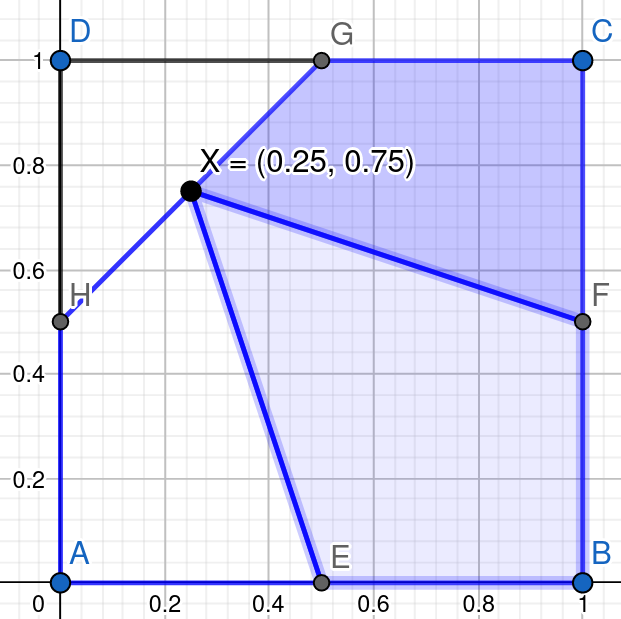
\includegraphics[width=0.3\textwidth]{image/farm.png}
\caption{$area(AEXH):area(BFXE):area(CGXF) = 2:3:2$}
\end{figure}

Please write a program to help Reed to determine whether it is possible to find the point
$X$ satisfying David's last will for a given set of numbers $p,q,r$.
If possible, please give a possible position of $X$ to Reed.
